%\begin{frame}[fragile]{Test tikz}
%
%
%    \begin{figure}[ht]
%        \begin{center}
%            \begin{tikzpicture}[auto, node distance=1cm,>=latex']
%            \node [input, name=input] {};
%            \node [sum, right=of input] (sum) {};
%            \node [block, right=of sum] (controller) {$C(s)$};
%            \node [block, right=2 of controller] (plant) {$G(s)$};
%            \node [output, right=of plant] (output) {};
%
%            \draw [draw,->] (input) -- node {$U(s)$} (sum);
%            \draw [->] (sum) -- node {} (controller);
%            \draw [->] (controller) -- node {} (plant);
%            \draw [->] (plant) -- node [name=y] {$Y(s)$}(output);
%            \draw [->] (y) -- ++ (0,-2) -| node [pos=0.99] {$-$} (sum);
%            \end{tikzpicture}
%        \end{center}
%    \end{figure}

%\end{frame}

%
\begin{frame}[t]{Motivácia: Počítače sú všade okolo nás...}
\begin{columns}
\begin{column}{.48\textwidth}
\begin{onlyenv}<1-2>
Text \cite{Cholodwicz2017}
\begin{figure}
\centering
  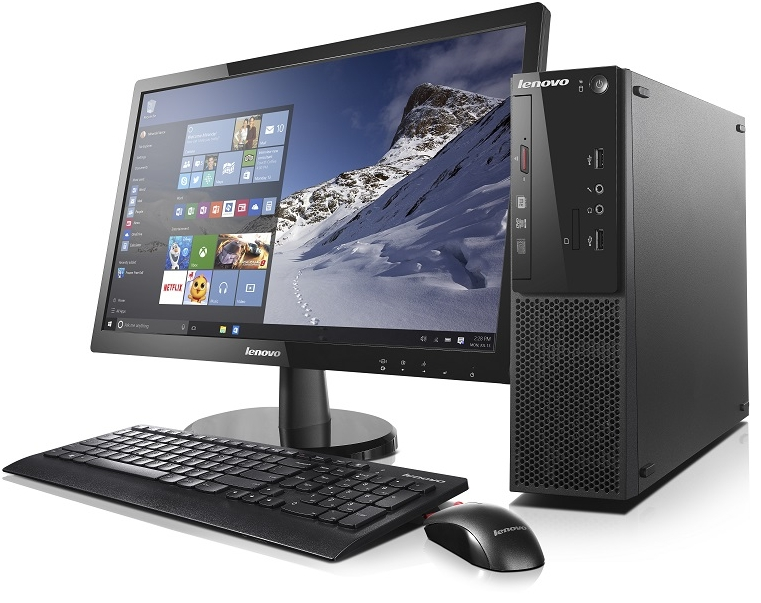
\includegraphics[height=55mm]{pc}\\
\end{figure}
\end{onlyenv}
\end{column}
\begin{column}{.48\textwidth}
\begin{onlyenv}<2>
\begin{figure}
\centering
  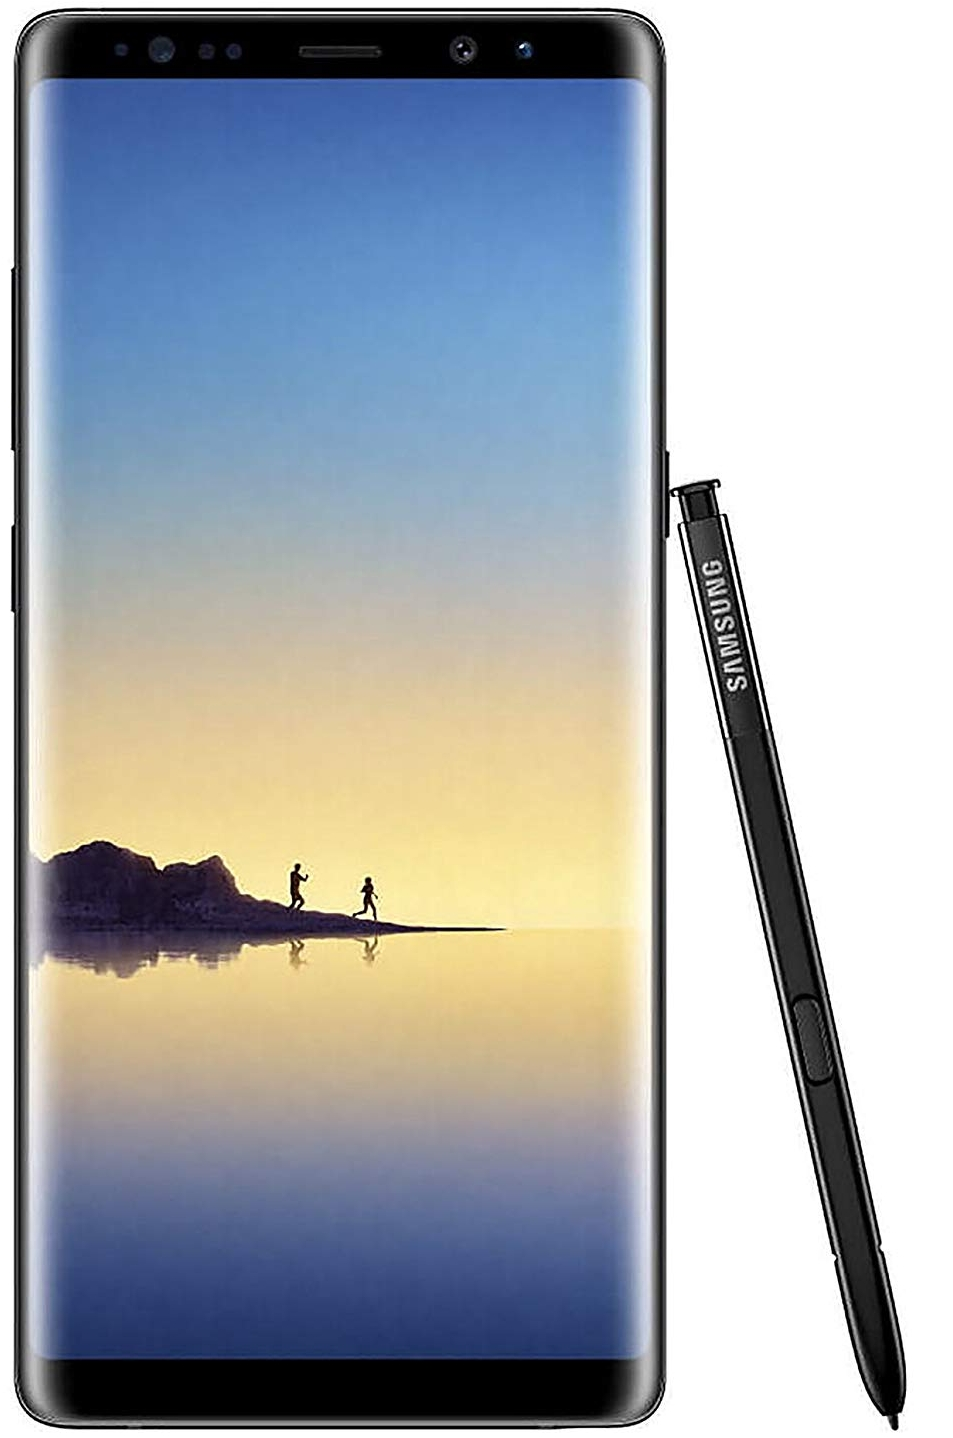
\includegraphics[height=55mm]{phone}\\
\end{figure}
\end{onlyenv}
\end{column}
\end{columns}
\end{frame}



\begin{frame}{Opakovanie: Riadená sústava}
  \begin{itemize}
    \item<1-> Riadená sústava, systém alebo proces \angl{plant, system, process}, v tomto prípade celá kvadrikoptéra
    \item<2-> Vstup $u(t)$ \angl{input} sú akčné zásahy, napr. PWM/RC do motorov
    \item<3-> Výstup $y(t)$ \angl{output} je meraná, tzv. manipulovaná veličina \angl{manipulated variable}; napr. klopenie $\theta(t)$ drona
    \item<4-> Porucha \angl{disturbance} $w(t)$ je vplyv vonkajšieho prostredia, napr. vietor
  \end{itemize}

\begin{figure}
\centering
  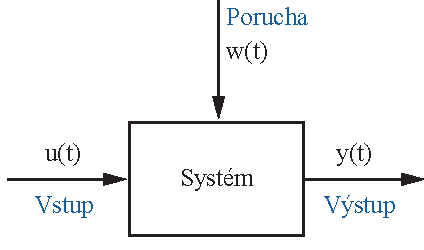
\includegraphics[width=60mm]{loop_1}\\
\end{figure}
\end{frame}

\begin{frame}{Opakovanie: Meranie}
  \begin{itemize}
    \item<1-> Výstupy $y(t)$ sú idealizované
    \item<2-> Poruchy, teda šum merania $v(t)$ a dynamika snímača vplýva na výsledok
    \item<3-> Merania môžeme korigovať, resp. nemerané veličiny odhadnúť $\hat{y}(t)$
    \item<4-> Pre jednoduchosť často predpokladáme ideálne meranie ${y}(t)=\hat{y}(t)$
  \end{itemize}

\begin{onlyenv}<1-3>
\begin{figure}
\centering
  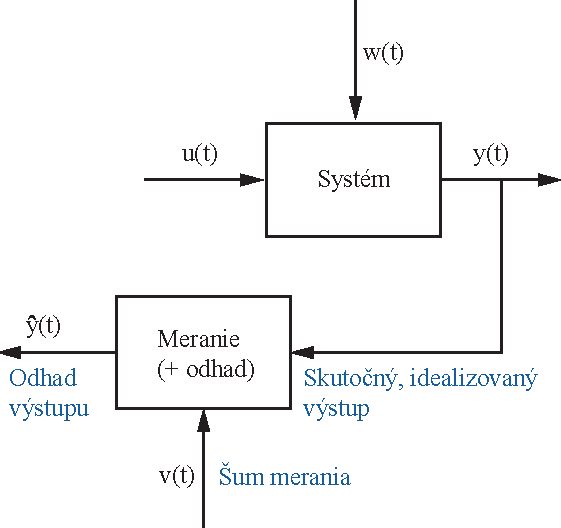
\includegraphics[width=60mm]{loop_2}\\
\end{figure}
\end{onlyenv}


\begin{onlyenv}<4>
\begin{figure}
\centering
  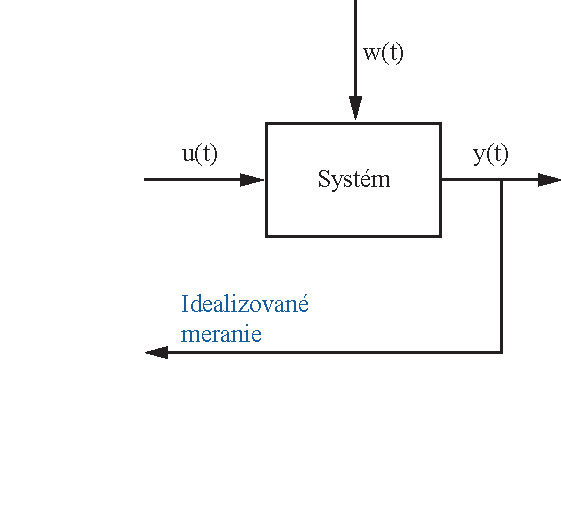
\includegraphics[width=60mm]{loop_2b}\\
\end{figure}
\end{onlyenv}
\end{frame}

\begin{frame}{Opakovanie: Riadiacia odchýlka}
  \begin{itemize}
    \item<1-> Žiadaná hodnota alebo referencia \angl{setpoint, reference} $r(t)$ vyjadruje na akú hodnotu chceme dostať výstup, potom
    \item<2-> Rozdiel medzi žiadanou hodnotou a výstupom $e(t)=r(t)-y(t)$ je odchýlka riadenia \angl{error}
  \end{itemize}

\begin{figure}
\centering
  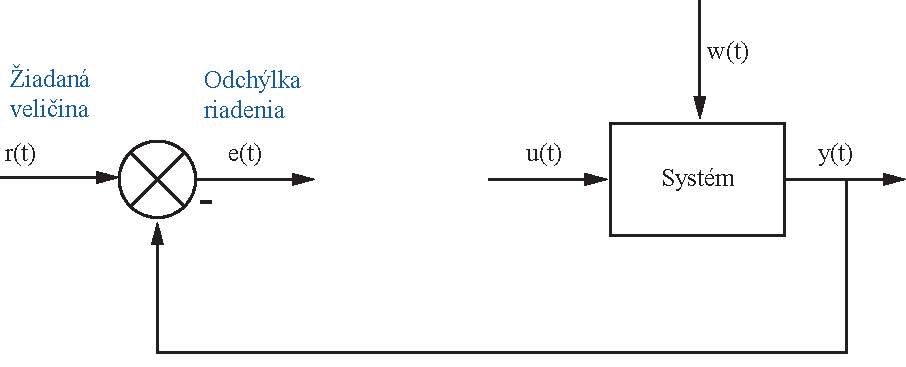
\includegraphics[width=100mm]{loop_ref}\\
\end{figure}
\end{frame}


\begin{frame}[t]{Opakovanie: Riadiaci algoritmus}
  \begin{itemize}
    \item<1-> Riadenie je logika ktorá prepočíta odchýlku riadenia $e(t)$ na vstupy $u(t)$
    \item<2-> Môže to byť ľubovoľné, do konca aj analógové a mechanické (e.g. riadenie rýchlosti parného stroja)
    \item<3-> Dobrým kompromisom medzi komplexnosťou (pochopenie, návrh) a implementovateľnosťou je PID riadenie
    \item<4-> Až 97\% riadiacich algoritmov v praxi sú PID... \citep{Murray2004}
    \item<5-> ...a väčšina z nich sú slabo naladené\footnote{ArduPilot: ``most heli users have not learned how to tune up their helis yet'' \citep{Hall2020}}
  \end{itemize}

\begin{onlyenv}<1>
\begin{figure}
\centering
  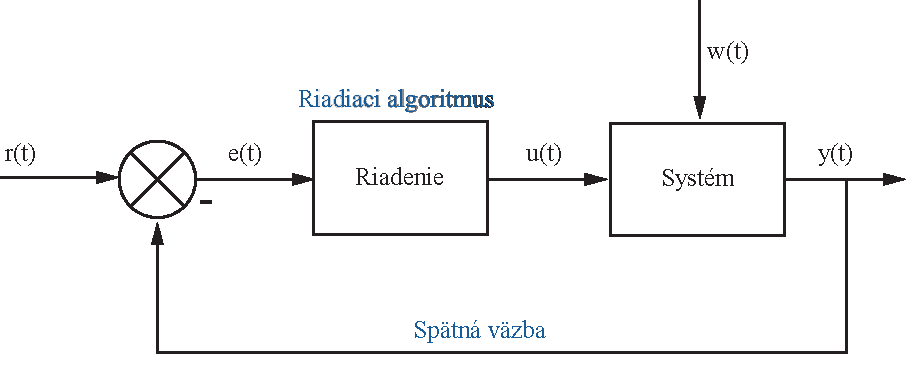
\includegraphics[width=80mm]{loop_all}\\
\end{figure}
\end{onlyenv}

\begin{onlyenv}<2>
\begin{figure}
\centering
  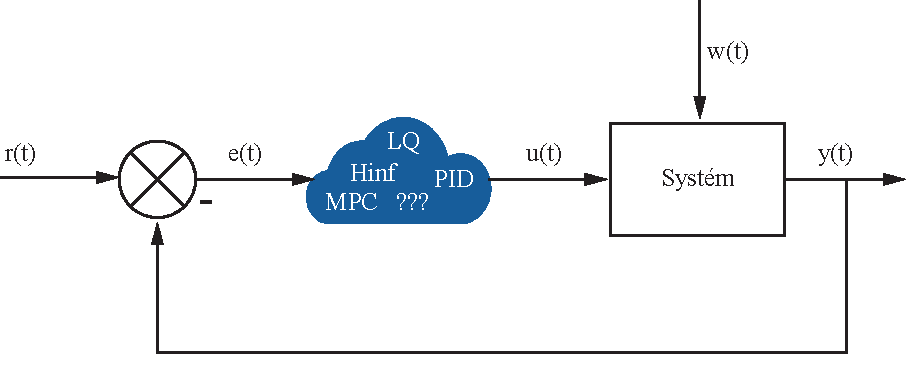
\includegraphics[width=80mm]{loop_Whatevs}\\
\end{figure}
\end{onlyenv}



\begin{onlyenv}<3->
\begin{figure}
\centering
  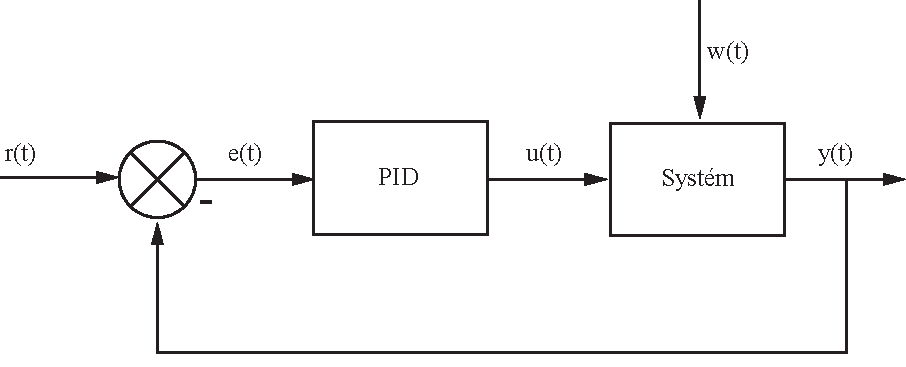
\includegraphics[width=80mm]{loop_PID}\\
\end{figure}
\end{onlyenv}
\end{frame}


\begin{frame}[t]{Opakovanie: PID}
  \begin{itemize}
    \item<1-> \textbf{Súčasnosť} = proporcionálna zložka: okamžitá odchýlka $e(t)$, ale majme možnosť na ladenie, tak $K_Pe(t)$.
    \item<2-> \textbf{Minulosť} = integračná zložka: celková odchýlka $e(t)$ v minulosti, ale majme možnosť na ladenie, tak $K_I\int_0^te(t)\mathrm{d}t$.
    \item<3-> \textbf{Budúcnosť} = derivačná zložka: projektovaná odchýlka $e(t)$ do budúcnosti, ale majme možnosť na ladenie, tak $K_D\frac{\mathrm{d}e(t)}{\mathrm{d}t}$.
  \end{itemize}

\begin{onlyenv}<1>
\begin{figure}
\centering
  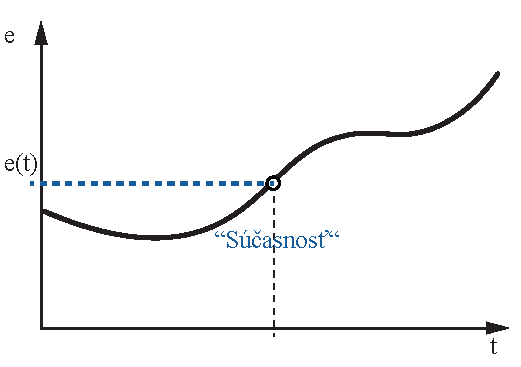
\includegraphics[width=50mm]{PID_P}\\
\end{figure}
\end{onlyenv}

\begin{onlyenv}<2>
\begin{figure}
\centering
  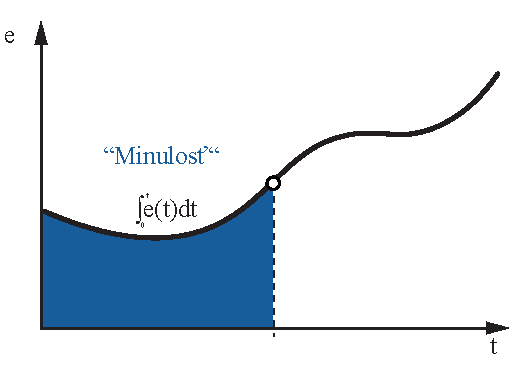
\includegraphics[width=50mm]{PID_I}\\
\end{figure}
\end{onlyenv}

\begin{onlyenv}<3>
\begin{figure}
\centering
  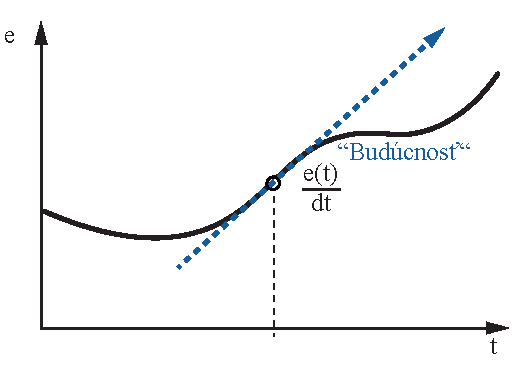
\includegraphics[width=50mm]{PID_D}\\
\end{figure}
\end{onlyenv}


\begin{onlyenv}<4->
tzv. paralelná (ideálna) forma
\begin{align}
u(t)= K_Pe(t)+K_I\int_0^te(t)\mathrm{d}t+K_D\frac{\mathrm{d}e(t)}{\mathrm{d}t}
\end{align}
\end{onlyenv}

\begin{onlyenv}<5>
alebo tzv. štandardná forma\footnote{V PX4 môžete prepínať pre rate controller \cite{PX4:PIDTuning}} (máme intuitívnejšie časové konštanty, ale zosilnenie je nezávislé\footnote{pozor, neintutívne...})
\begin{align}
u(t)= K_P\left(e(t)+\frac{1}{T_I}\int_0^te(t)\mathrm{d}t+T_D\frac{\mathrm{d}e(t)}{\mathrm{d}t}\right)
\end{align}
\end{onlyenv}
\end{frame}




\begin{frame}[t]{Opakovanie: Vzorkovanie, tvarovanie}
  \begin{itemize}
  \item<1-> Výpočtová realizácia neumožní počítať spojito, preto
    \begin{itemize}
      \item Vzorkujeme na strane výstupov --- ADC + slučka v hard real-time pomocou časovačov
      \item Tvarujeme na strane vstupov --- zero order hold (ZOH) len znamená podržíme hodnotu počas vzorky
    \end{itemize}
  \item<2-> Vzorkovanie mení spojitý čas na $t=kT_s$. Perióda je voliteľná, ale
    \begin{itemize}
      \item musí zachytiť dominantnú dynamiku riadeného deja,
      \item a výpočtová realizácia musí stíhať.
  \end{itemize}
\end{itemize}
\begin{figure}
\centering
  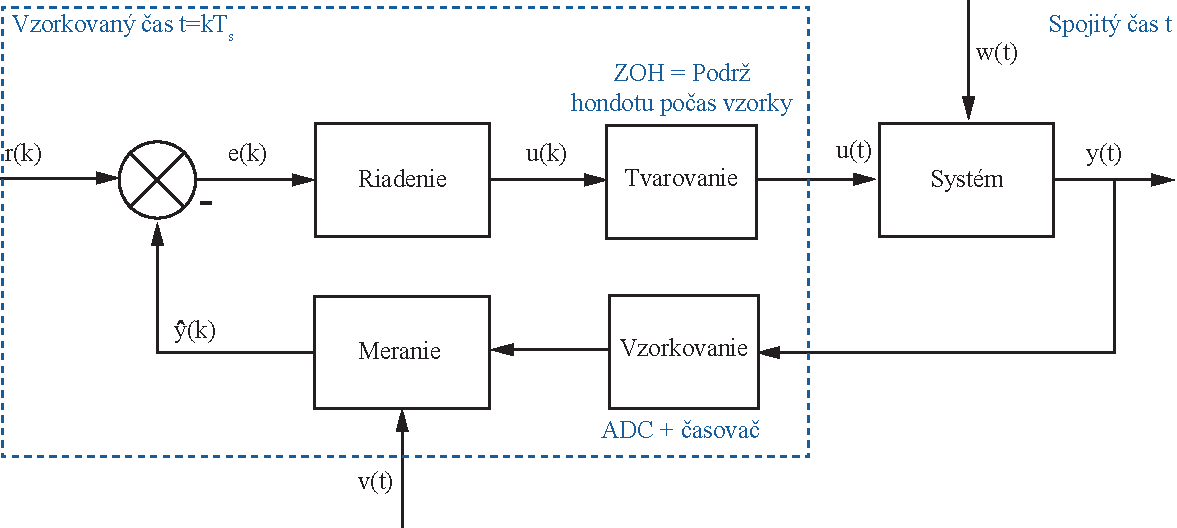
\includegraphics[width=0.9\textwidth]{loop_Sampling}\\
\end{figure}
\end{frame}


\begin{frame}[t]{Opakovanie: Číslicové PID}
  \begin{itemize}
    \item<1-> Systém, resp. proces zostáva spojitý\footnote{Samozrejme máme aj nespojité procesy a systémy}
    \item<2-> Koncepty ako integrácia, derivácia musíme numericky aproximovať, t.j. ak $T_s$ je vzorkovací čas, naše PID bude
        \begin{align}
        u(k)= K_Pe(k)+K_I\underbrace{\sum_0^te(k)T_s}_{\mathrm{``obdlzniky''}}+K_D\underbrace{\frac{e(k)-e(k-1)}{T_s}}_{\mathrm{``vstupanie''}}
        \end{align}
    \item<3->  alebo v prakticky vhodnejšej tzv. inkrementálnej forme pre MCU (bez dôkazu, viď. \cite{W:PID})
        {\scriptsize
        \begin{align}
        u(k)=u(k-1)+\left(K_P+K_IT_s+\frac{K_D}{T_s}\right)e(k)+\left(-K_P -2\frac{K_D}{T_s}\right)e(k-1)+\frac{K_D}{T_s}e(k-2)
         \end{align}
         }
\end{itemize}
\end{frame}




%\begin{frame}{Opakovanie: Riadená sústava}
%  \begin{itemize}
%    \item<1-> blah
%    \item<2-> blah blah
%  \end{itemize}

%%\begin{onlyenv}<1>
%\begin{figure}
%\centering
%  \includegraphics[width=\textwidth]{loop_full}\\
%\end{figure}
%%\end{onlyenv}
%\end{frame}
% 